\scanpage{341}

Bien sûr, ce caractère s'appelera encore, ``multiplicateur'', \unsure{et|ou} ``caractère cyclotomique''. \deleted{\unsure{Il}} Si notre conjecture fondamentale est vraie, ce caractère identifie $(\Gamma_\Sigma)_{\mathrm{ab}}$ à $\widehat{\mathbb Z}^{*}$.

Par contre, si $I=I(\pi)$, l'hom canonique
\[
\widehat{\widehat{\mathcal T}}\longrightarrow\unsure{\mathfrak S_I|\mathcal S_I}
\]
n'est \deleted{\illegible{1}} pas trivial sur $\Sigma$, mais induit un hom surjectif
\[
\Sigma\longrightarrow\mathfrak S_I^{\deleted{\unsure{!}}}
\]
d'où un sous-groupe $\Sigma^!$ tel que
\[
\Sigma/\Sigma^!\xrightarrow{\sim}\mathfrak S_I.
\]
\margin{\unsure{moralement}, $\Sigma^!\simeq\widehat{\mathcal T}^{!+}$}

On voit de suite que $\forall\ \unsure{\gamma|g}\in\widehat{\widehat{\mathcal T}}$ qui normalise $\Sigma$ normalise $\Sigma^!=\Sigma\cap\widehat{\widehat{\mathcal T}}^!$, \unsure{d'où|i.e.} $\Sigma^!$ est aussi invariant dans $\mathcal N_\Sigma$. \deleted{\illegible{3}} Soit $\mathcal N_\Sigma^!=\mathcal N_\Sigma\cap\widehat{\widehat{\mathcal T}}^!$, on a un diagramme cartésien de ss-groupes de $\widehat{\widehat{\mathcal T}}$
\diagram{\begin{tikzcd}[ampersand replacement=\&]
\mathcal N^!\arrow[r,hook,"\mathfrak S_I"] \& \mathcal N\\
\Sigma^!\arrow[u,hook,"\Gamma_\Sigma"]\arrow[r,hook,"\mathfrak S_I"'] \& \Sigma\arrow[u,hook,"\Gamma_\Sigma"']
\end{tikzcd}}
donnant un hom injectif
\[
\mathcal N/\Sigma^!\longrightarrow
\underbrace{\mathcal N/\mathcal N^!}_{\mathfrak S_I}\times
\underbrace{\mathcal N/\Sigma}_{\Gamma_\Sigma}
\]
\unsure{dont|quand} on voit de suite qu'il est bijectif
\margin{\unsure{et|car} $\unsure{\Sigma}/\Sigma^!\xrightarrow{\sim}\mathcal N/\mathcal N^!\ (\simeq\mathfrak S_I)$}
\[
\mathcal N/\Sigma^!\xrightarrow{\sim}\mathcal N/\mathcal N^!\times\mathcal N/\Sigma\simeq\mathfrak S_I\times\Gamma_\Sigma
\]
et on a par suite aussi
\[
\unsure{\mathcal N}^!/\Sigma^!\xrightarrow{\sim}\mathcal N/\unsure{\Sigma}=\Gamma_\Sigma,
\]
i.e. le groupe $\Gamma_\Sigma$ des autom \unsure{arithmétiquement} ext. de $(\pi,\Sigma)$ peut se décrire aussi via les automs.
\mspage{340}

\scanpage{342}
\mspage{173}

extérieurs induisant l'identité sur $I$.

Dans le cas $(g,\nu)=(0,3)$, on a $\Sigma^!=(1)$, \unsure{$\Rightarrow$} donc $\Sigma\xrightarrow{\sim}\mathfrak S_3$. $\mathcal N$ est le \deleted{produit} normalisateur de $\mathfrak S_3$ dans $\widehat{\widehat{\mathcal T}}$, $\mathcal N^!$ \inserted{$\unsure{\xrightarrow{\sim}}\Gamma_\Sigma$} est son centralisateur, et $\mathcal N$ s'identifie au produit direct des deux.

\deleted{\illegible{2}}

Soit maintenant $\unsure{I|I'}\subset I$, \inserted{$\nu'=\operatorname{card}I'$,} et considérons le groupe extérieur $\pi'$ déduit de $\pi$ par ``bouchage des trous en $\unsure{I\setminus I'}$'', d'où hom
\[
\pi^{\unsure{*}}\longrightarrow\pi'.
\]
\deleted{\unsure{Pour une application}} \inserted{Considérons} les bases \inserted{de $\pi$,} pour lesquelles \deleted{$l_{\nu-\nu'+1}\ldots l_\nu$} \deleted{\illegible{2}} \inserted{les $\nu'$ \deleted{derniers} \inserted{premiers} $l_i$,} soient dans des \inserted{\deleted{\unsure{bases}}} groupes \unsure{à} lacets \deleted{\unsure{dans}} $L_{i'}$ $(i'\in I')$ --- on les appelle adaptées à $I'$; elles forment un torseur \inserted{$\subset\operatorname{Isom}_{\mathrm{lac}}(\widehat\pi_{g,\nu},\pi)$} sous le sous-groupe de \deleted{\illegible{1}} $\unsure{\widehat{\widehat{\mathcal G}}}_{g;(\nu,\nu'\deleted{\unsure{+2}})}$ de $\widehat{\widehat{\mathcal G}}_{g,\nu}$ \inserted{$=\operatorname{Aut}\deleted{\,\mathrm{ext}}_{\unsure{\mathrm{lac}}}(\widehat\pi_{g,\nu})$} \inserted{formé} des $\unsure{u|h}\in\widehat{\widehat{\mathcal G}}_{g,\nu}$ dont l'image dans $\mathfrak S_I$ \unsure{invarie} \inserted{\deleted{\unsure{aussi}} l'ens} des $\nu'\deleted{\unsure{+2}}$ premiers éléments (\unsure{ou}, des $\nu-\unsure{\nu'}$ derniers \inserted{\unsure{son|leur} ens complémentaire,}).

\margin{D'où aussi : $\forall$ base, $\forall$ discrétification, discrétification orientée de $\pi$ en définit une de $\pi'$, d'où \unsure{itou} pour classes de \inserted{$\pi,\pi'$} conjugaison, i.e. \unsure{pour|par} les prédiscrétifications \inserted{(év. orientées)} strictes, et aussi \unsure{pour|par} les adhérences des classes, i.e. les \deleted{\illegible{1}} prédiscrétifications et prédiscrétifications orientées. Il n'y a que le cas des \unsure{arithmétis.|arithmétisations} qui \deleted{\unsure{demande}} \inserted{\unsure{demanderait}} une analyse plus fine\ldots}

Pour une telle base, on trouve une base correspondante de $\pi'$. \deleted{le passage} La donnée de $(\pi,I')$ équivaut à celle d'un torseur sous $\widehat{\widehat{\mathcal G}}_{g,(\nu,\nu'\deleted{\unsure{+2}})}$, celle d'un $\pi'$ à \deleted{\illegible{1}} la donnée d'un torseur sous $\widehat{\widehat{\mathcal G}}_{g,\nu'}$, et le passage de $\pi$ à $\pi'$ se décrit par le chgt de groupe d'opérateurs
\[
\widehat{\widehat{\mathcal G}}_{g,(\nu,\nu')}\longrightarrow\widehat{\widehat{\mathcal G}}_{g,\nu'}
\]
cet homomorphisme envoie $\underset{\inserted{\substack{\cap\\ \Sigma_{g,\nu}}}}{\widehat{\mathcal G}_{g,(\nu,\nu')}}\inserted{=\Sigma_{g,(\nu,\nu')}}$ dans $\unsure{\widehat{\mathcal G}}_{g,\nu'}=\Sigma_{g,\nu'}$,
\mspage{341}

\scanpage{343}

\inserted{et $\overline{\mathrm m}$} $\mathcal G_{g,(\nu,\nu')}$ dans $\mathcal G_{g,\nu'}$, aussi $\pi$ dans $\pi'$. Il s'ensuit que toute prédiscrétification de $\pi$ en définit une de $\pi'$, de $\overline{\mathrm m}$ pour les prédiscrétifications strictes, \deleted{bases} discrétifications, bases extérieures \inserted{``adaptées à $I'$'' \deleted{\unsure{(i.e.) pour lesquelles}}}. Enfin, si on a une ``préarithmétisation'' de $\pi$, i.e. un $\Sigma\subset\widehat{\widehat{\mathcal T}}(\pi)$, en déduit-on une préarithmétisation de $\pi'$ --- i.e. \inserted{\unsure{(p.ex.)}} si deux prédiscrétifications de $\pi$ sont compatibles i.e. \deleted{\unsure{définissent}} ont le $\overline{\mathrm m}$ groupe $\Sigma\subset\widehat{\widehat{\mathcal T}}(\pi)\unsure{,}$ d'autom extérieurs, en est-il de $\overline{\mathrm m}$ de leurs images ?

\deleted{\unsure{[}La question revient à celle-ci :\unsure{]}
\unsure{[}l'hom
\[
\widehat{\widehat{\mathcal T}}_{g,(\nu,\nu')}
\longrightarrow\widehat{\widehat{\mathcal T}}_{g,\nu'},
\]
\unsure{qui envoie}
\[
\widehat{\mathcal T}_{g,(\nu,\nu')}=\unsure{\Sigma}_{g,(\nu,\nu')}
\]
dans]}

Pour y voir plus clair, on va écrire sous forme de diagrammes les ens. remarquables associés à $\pi$, et ceci de deux façons, l'une sans utiliser de \unsure{structure particulière|structures particulières} sur $I=I(\pi)$, l'autre en utilisant un ordre total, ce qui permet, dans le torseur $\operatorname{Isom}_{\mathrm{lac}}(\widehat\pi_{g,\nu},\pi)$ sous $\widehat{\widehat{\mathcal G}}_{g,\nu}$, de définir le sous-torseur sous $\widehat{\widehat{\mathcal G}}_{g,\nu}^{!}$ qu'on peut noter \deleted{\illegible{1}} $\operatorname{Isom}_{\mathrm{lac}}^{!}(\widehat\pi_{g,\nu},\pi)$.
\mspage{342}

\scanpage{344}
\mspage{174}

\diagram{
\begin{tikzcd}[ampersand replacement=\&,column sep=large,row sep=large]
\& \&
\begin{gathered}
\text{Bases de }(\pi)\simeq\operatorname{Isom}_{\mathrm{lac}}(\widehat{\pi}_{g,\nu},\pi)\\
\downarrow\\
[\text{Bases}^{!}(\pi)\simeq\operatorname{Isom}^{!}_{\mathrm{lac}}(\widehat{\pi}_{g,\nu},\pi)]
\end{gathered}
\arrow[dl,"\mathcal G^{+}_{g,\nu}"']\arrow[dr,"\widehat{\pi}_{g,\nu}"]
\&\\
\&
\begin{gathered}
\text{discrétifications}\ \inserted{\text{orientées}}\ (\pi)\\
\simeq\operatorname{Isom}_{\mathrm{lac}}(\widehat{\pi}_{g,\nu},\pi)/\mathcal G^{+}_{g,\nu}\\
\simeq\operatorname{Isom}^{!}_{\mathrm{lac}}(\widehat{\pi}_{g,\nu},\pi)/\mathcal G^{!+}_{g,\nu}
\end{gathered}
\arrow[dl,"\{\pm1\}"']\arrow[dr]
\&\&
\begin{gathered}
\text{Bases extérieures de }\pi\\
\simeq\operatorname{Isom}\deleted{\,\mathrm{ext}}_{\mathrm{lac}}(\widehat{\pi}_{g,\nu},\pi)/\widehat{\pi}_{g,\nu}\\
\simeq\operatorname{Isom\,ext}_{\mathrm{lac}}(\widehat{\pi}_{g,\nu},\pi)\\
\downarrow\\
[\text{Bases ext}^{!}(\pi)\simeq\operatorname{Isom\,ext}^{!}_{\mathrm{lac}}(\widehat{\pi}_{g,\nu},\pi)]
\end{gathered}
\arrow[dl,"\mathcal T_{g,\nu}"]\\
\left[\begin{gathered}\text{Discrétifications }(\pi)\\\simeq\end{gathered}\right]
\arrow[d]
\&\&
\begin{gathered}
\text{prédiscrétifications}\ \inserted{\text{orientées}}\ \text{strictes}\ (\pi)\\
\simeq\operatorname{Isom}_{\mathrm{lac}}(\unsure{\widehat{\pi}}_{g,\nu},\pi)/\mathcal G^{+}_{g,\nu}\cdot\widehat{\pi}_{g,\nu}\\
\simeq\operatorname{Isom\,ext}_{\mathrm{lac}}(\widehat{\pi}_{g,\nu},\pi)/\mathcal T^{+}_{g,\nu})\\
\simeq\operatorname{Isom}^{!}(\widehat{\pi}_{g,\nu},\pi)/\mathcal G^{!+}_{g,\nu}\cdot\widehat{\pi}_{g,\nu}\\
\simeq\operatorname{Isom\,ext}_{\mathrm{lac}}(\widehat{\pi}_{g,\nu},\pi)/\mathcal T^{!+}_{g,\nu}
\end{gathered}
\arrow[dll,"\{\pm1\}"']\arrow[d]
\&\\
\left[\begin{gathered}\text{prédiscrétifications strictes}\\\text{de }\pi\\\simeq\end{gathered}\right]
\&\&
\begin{gathered}
\text{prédiscrétifications}\ \inserted{\text{orientées}}\ (\pi)\\
\simeq\operatorname{Isom}_{\mathrm{lac}}(\widehat{\pi}_{g,\nu},\pi)/\widehat{\mathcal G}^{+}_{g,\nu}\\
\simeq\operatorname{Isom\,ext}_{\mathrm{lac}}(\widehat{\pi}_{g,\nu},\pi)/\widehat{\mathcal T}^{+}_{g,\nu}\\
\deleted{\unsure{\simeq}}\quad
\simeq\operatorname{Isom}^{!}_{\mathrm{lac}}(\widehat{\pi}_{g,\nu},\pi)/\widehat{\mathcal G}^{!+}_{g,\nu}\\
\simeq\operatorname{Isom\,ext}^{!}_{\mathrm{lac}}(\widehat{\pi}_{g,\nu},\pi)/\widehat{\mathcal T}^{!+}_{g,\nu}
\end{gathered}
\arrow[dll,"\{\pm1\}"']\arrow[dd,"\Gamma_{\Sigma}"',"\Gamma_{g,\nu}"]
\&\\
\left[\begin{gathered}\text{prédiscrétifications de }\pi\\\simeq\end{gathered}\right]
\arrow[drr]
\&\&\&\\
\&\&
\begin{gathered}
\text{préarithmétisations de }\pi\\
\simeq\operatorname{Isom}_{\mathrm{lac}}(\widehat{\pi}_{g,\nu},\pi)/\mathcal M_{g,\nu}\\
\simeq\operatorname{Isom\,ext}_{\mathrm{lac}}(\widehat{\pi}_{g,\nu},\pi)/\mathcal N_{g,\nu}\\
\simeq\operatorname{Isom}^{!}_{\mathrm{lac}}(\widehat{\pi}_{g,\nu},\pi)/\mathcal M^{!}_{g,\nu}\\
\simeq\operatorname{Isom\,ext}^{!}_{\mathrm{lac}}(\widehat{\pi}_{g,\nu},\pi)/\mathcal N^{!}_{g,\nu}
\end{gathered}
\&
\end{tikzcd}
}

\margin{\unsure{pas séparé}}
\margin{\unsure{pas séparé}}
\margin{\diagram{\begin{tikzcd}[ampersand replacement=\&]
\deleted{\left\downarrow\vphantom{\rule{0pt}{2.8cm}}\right.}
\end{tikzcd}}}
\margin{\diagram{\begin{tikzcd}[ampersand replacement=\&,column sep=0.35cm,row sep=1.4cm,cells={nodes={inner sep=0pt,minimum size=0pt}}]
{} \& {} \arrow[d,bend right=8,line width=0.8pt,
  "{\widehat{\mathcal T}_{g,\nu}}"{pos=0.95,right}] \\
{} \& {} \arrow[dl,bend right=8,no head,line width=0.3pt] \\
{} \& {}
\end{tikzcd}}}
\margin{\diagram{\begin{tikzcd}[ampersand replacement=\&,column sep=0.30cm,row sep=0.40cm,cells={nodes={inner sep=0pt,minimum size=0pt}},arrows={line width=0.65pt,start anchor=center,end anchor=center,shorten <=1.2pt,shorten >=1.2pt}]
{} \& {} \& {} \arrow[dl] \arrow[dr] \& {} \& {} \arrow[ll] \arrow[dr] \& {} \\
|[yshift=-0.05cm]| {} \arrow[dr] \& {} \arrow[l] \arrow[dr] \& {} \& {} \arrow[dl] \& {} \& {} \arrow[ll] \\
{} \& |[yshift=-0.04cm]| {} \arrow[d] \& {} \arrow[l] \arrow[d] \& {} \& {} \& {} \\
{} \& |[yshift=-0.06cm]| {} \arrow[dr] \& {} \arrow[l] \arrow[dd,line width=1.25pt] \& {} \& {} \& {} \\
{} \& {} \& |[xshift=-0.12cm,yshift=-0.25cm]| {} \& {} \& {} \& {} \\
{} \& {} \& |[yshift=-0.45cm]| {} \& {} \& {} \& {}
\end{tikzcd}}}
\margin{TSVP}
\mspage{343}

\scanpage{345}

\uline{NB}

On pose \deleted{\illegible{1}}
\[
\Gamma_{g,\nu}=\mathcal N_{g,\nu}/\Sigma_{g,\nu}
=\mathcal N^{!}_{g,\nu}/\Sigma^{!}_{g,\nu}
\]
(où $\Sigma_{g,\nu}=\widehat{\mathcal T}^{+}_{g,\nu}$,
$\Sigma^{!}_{g,\nu}=\widehat{\mathcal T}^{!+}_{g,\nu}$).
On peut aussi le décrire comme le groupe $\Gamma_{\Sigma}$ associé à un
groupe \inserted{ext} profini à lacets \inserted{$\pi$}
\uline{muni} d'une prédiscrétification \inserted{orientée}
$\alpha$ (sans plus). Si on a deux tels \deleted{groupes}\inserted{couples}
$(\pi,\alpha),(\pi',\alpha')$, \unsure{d'où} $\Gamma_{\Sigma}$ et
$\Gamma_{\Sigma'}$ ($\Sigma=\operatorname{Aut\,ext}_{\mathrm{lac}}(\pi,\alpha)$,
$\Sigma'=\operatorname{Aut\,ext}_{\mathrm{lac}}(\pi',\alpha')$), on trouve en effet un
isom. \uline{can.}
\[
\Gamma_{\Sigma}\xrightarrow{\sim}\Gamma_{\Sigma'}
\]
en prenant n'importe quel isom ext. \inserted{à lacets $u$} de $\pi$ avec $\pi'$,
transformant $\alpha$ en $\alpha'$ --- l'isom associé
$\Gamma_{\Sigma}\longrightarrow\Gamma_{\Sigma'}$ ne dépend évidemment pas du choix de
$u$.

Ceci posé, les \inserted{couples $(\pi,\Sigma)$ d'un}
\unsure{groupe|groupes} \unsure{profini|profinis} à lacets de type $(g,\nu)$,
\deleted{munis d'une}\inserted{\unsure{muni d'une}} préarithmétisation,
avec comme morphismes les \unsure{isomorphismes} \unsure{arithmétiquement} extérieurs
\deleted{transformant}\inserted{(relatifs à} $\Sigma$ et $\Sigma'\ldots$),
forment un groupoïde connexe $\Pi_{g,\nu}$, ayant un objet ``origine''
(défini à isom unique près comme étant $(\widehat{\pi}_{g,\nu},\Sigma_{g,\nu})$,
\unsure{ou au choix} n'importe quel $(\pi,\Sigma_{\alpha})$ provenant d'un
$(\pi,\alpha)$ ($\alpha$ une prédiscrétification orientée de $\pi$),
et dont le groupe \unsure{des} \unsure{autom} est justement $\Gamma_{g,\nu}$.
\mspage{344}

\scanpage{346}
\mspage{175}

On constate que, à l'exception des deux espaces homogènes
(sous $\widehat{\widehat{\mathcal G}}(\pi)$, mais pas \unsure{nécess|néc} sous
$\widehat{\widehat{\mathcal G}}(\pi,I')$, voire sous
$\widehat{\widehat{\mathcal G}}^{!}(\pi)$) Bases $(\pi)$ et Bases ext $(\pi)$,
les quatre autres sont en fait des espaces homogènes sous
$\widehat{\widehat{\mathcal G}}^{!}$, et s'expriment comme quotients du
\inserted{$\widehat{\widehat{\mathcal G}}^{!}_{g,\nu}$-}torseur
$\operatorname{Isom}^{!}(\widehat{\pi}_{g,\nu},\pi)$, par les quatre sous-groupes
\[
\mathcal G^{!}_{g,\nu},\quad
\mathcal G^{!}_{g,\nu}\cdot\widehat{\pi}_{g,\nu},\quad
\widehat{\mathcal G}^{!}_{g,\nu},\quad
\mathcal M^{!}_{g,\nu}
\]
(le dernier défini comme image inverse de $\mathcal N^{!}_{g,\nu}$ dans
$\widehat{\widehat{\mathcal G}}_{g,\nu}$, tt comme $\mathcal M_{g,\nu}$ est défini
comme image inverse de $\mathcal N_{g,\nu}$).
On trouve d'autre part, \unsure{si|à} $I'=\{i_0,\ldots,i_{\nu'-1}\}$,
\unsure{un|des} hom.
\[
\widehat{\widehat{\mathcal G}}^{!}_{g,\nu}\longrightarrow
\widehat{\widehat{\mathcal G}}^{!}_{g,\nu'},
\]
envoyant $\mathcal G^{!}_{g,\nu}$ dans $\mathcal G^{!}_{g,\nu'}$,
\deleted{\illegible{1} $\unsure{\widehat{\mathcal G}}_{g,\nu}$ dans
$\unsure{\widehat{\pi}_{g,\nu}}$}
en envoyant $\pi_{g,\nu}$ dans $\pi_{g,\nu'}$, donc $\widehat{\pi}_{g,\nu}$
dans $\widehat{\pi}_{g,\nu'}$,
$\widehat{\mathcal G}^{!}_{g,\nu}=\Sigma^{!}_{g,\nu}$ dans
$\widehat{\mathcal G}^{!}_{g,\nu'}=\Sigma^{!}_{g,\nu'}$, et le sous-groupe
$\mathcal G^{!}_{g,\nu}\cdot\widehat{\pi}_{g,\nu}$ de
\deleted{\illegible{1}} \inserted{$\widehat{\mathcal G}^{!}_{g,\nu}$}
dans le sous-groupe $\mathcal G^{!}_{g,\nu'}\cdot\widehat{\pi}_{g,\nu'}$ de
$\widehat{\mathcal G}^{!}_{g,\nu'}$.
Enfin, comme $\Sigma^{!}_{g,\nu}$ s'envoie dans $\Sigma^{!}_{g,\nu'}$,
\deleted{\illegible{1}} $\mathcal N^{!}_{g,\nu}$ s'envoie dans le normalisateur
de $\Sigma^{!}_{g,\nu'}$ \inserted{(dans $\widehat{\widehat{\mathcal T}}^{!}_{g,\nu'}$)},
\deleted{qui}\inserted{je dis que ce} n'est autre que $\mathcal N^{!}_{g,\nu'}$.
Changeant de notation, ceci revient au

\uline{Lemme}\quad Le
$\mathcal N^{!}_{\Sigma}=\operatorname{Norm}_{\widehat{\widehat{\mathcal T}}^{!}}(\Sigma^{!})$
\deleted{\illegible{1}}
$\bigl(=\operatorname{Norm}_{\widehat{\widehat{\mathcal T}}}(\Sigma^{!})\cap
\widehat{\widehat{\mathcal T}}^{!}\bigr)$.

\margin{pas prouvé\quad
\deleted{\illegible{4} de
$\unsure{\operatorname{Norm}_{\widehat{\widehat{\mathcal T}}}(\Sigma^{!})/\Sigma^{!}}$}}

Evidemment on a
$\mathcal N^{!}_{\Sigma}\subset
\operatorname{Norm}_{\widehat{\widehat{\mathcal T}}}(\Sigma^{!})\cap
\widehat{\widehat{\mathcal T}}^{!}$,
inversement soit $g\in\widehat{\widehat{\mathcal T}}^{!}$ qui normalise
$\unsure{\Sigma^{!}}$, montrons qu'il normalise $\Sigma$ i.e.
qu'il \unsure{est} $\in\mathcal N$
(donc $\in\mathcal N^{!}=\mathcal N\cap\widehat{\widehat{\mathcal T}}^{!}$).
\mspage{345}

\scanpage{347}

C'est pas clair. J'ai \inserted{pourtant} envie de \unsure{prouver|prononcer} \deleted{\illegible{1}} la
\uline{conjecture} L'application canonique
\[
\unsure{\text{Prédiscrét}|\text{Prédiscrit}}^{+}(\pi)
 \overset{\sim}{\longrightarrow}
\unsure{\text{Prédiscrét}|\text{Prédiscrit}}^{+}(\pi')
\]
est \uline{bijective}. Pour \inserted{que} deux prédiscrétifications \unsure{orientées}
$\alpha,\beta$ de $\pi$ \deleted{\unsure{soient}} \unsure{aient} $\overline{\mathrm m}$ groupe d'\unsure{autom.} extérieurs
$\Sigma_\alpha=\Sigma_\beta$, \deleted{alors} il faut et \unsure{s.}
\deleted{\unsure{pour leurs im.}} \inserted{qu'il en soit ainsi.}
pour leurs images $\Sigma_{\alpha'}$ et $\Sigma_{\beta'}$, i.e. que
$\Sigma_{\alpha'}=\Sigma_{\beta'}$; de sorte que la bijection précédente induit une bijection
\[
\text{Préarithm.}(\pi)\overset{\sim}{\longrightarrow}\text{Préarithm.}(\pi').
\]
Enfin, \deleted{l'application $\widehat{\widehat{\mathcal T}}(\pi)\longrightarrow
\widehat{\widehat{\mathcal T}}(\pi')$, qui induit}
\inserted{les bijections précédentes sont compatibles avec}
l'hom. des groupes \inserted{d'opérateurs}
$\widehat{\widehat{\mathcal T}}(\pi,I')\longrightarrow\widehat{\widehat{\mathcal T}}(\pi')$,
\deleted{\unsure{qui induit}} \inserted{a fortiori}
un $\widehat{\widehat{\mathcal T}}^{!}(\pi)\longrightarrow\widehat{\widehat{\mathcal T}}^{!}(\pi')$,
\deleted{ce} qui implique \unsure{qu'il en induit|qu'il les induit}
(pour une préarithmétisation $\Sigma$ \inserted{$\subset\widehat{\widehat{\mathcal T}}(\pi)$}
donnée de $\pi$, donnant $\Sigma'$ \inserted{$\subset\widehat{\widehat{\mathcal T}}(\pi')$}
dans $\pi'$; \inserted{avec $\Sigma^{!}\longrightarrow\Sigma'^{!}$}) un
hom.
$\mathcal N_\Sigma^{!}\deleted{\unsure{(\Sigma)}}\longrightarrow
\mathcal N_{\Sigma'}^{!}\deleted{\unsure{(\Sigma')}}$,
\deleted{\unsure{qui est de $\overline{\mathrm m}$}} et l'hom. \unsure{correspondant}
\[
\Gamma_\Sigma=\deleted{\illegible{1}}\mathcal N_\Sigma^{!}/\Sigma^{!}
 \longrightarrow
\deleted{\unsure{\mathcal N_{\Sigma'}^{!}/\Sigma'^{!}}}\Gamma_{\Sigma'}=\mathcal N_{\Sigma'}^{!}/\Sigma'^{!}
\]
est un isomorphisme.

Pour s'en convaincre il suffit de regarder
\deleted{\unsure{$\pi=\widehat{\pi}_{g,\nu}$}}
\inserted{(\unsure{choisissant} $\pi=\unsure{\pi_{g,\nu}|\widehat{\pi}_{g,\nu}}$,
$I'$ \deleted{\illegible{1}} \unsure{réduit au|étant un} dernier \unsure{élémt|élément} de $I_\nu$)}
le cas où $I'=\{\unsure{i'|i}\}$, On a alors un hom.
\[
\widehat{\widehat{\mathcal T}}(\pi,i)\longrightarrow
\widehat{\widehat{\mathcal G}}(\pi').
\]
(les autom. \uline{ext.} à lacets de $\pi$ fixant $i$ définissent des
\unsure{autom.} bien déterminés de $\pi'$ --- pas seulement extérieurs)
\mspage{346}

\scanpage{348}
\mspage{176}

i.e. $\widehat{\widehat{\mathcal G}}(\pi,i)\longrightarrow
\widehat{\widehat{\mathcal G}}(\pi')$ est trivial sur $\unsure{\widehat{\pi}}$, et
passe donc en quotient un
$\widehat{\widehat{\mathcal T}}(\pi,i)\longrightarrow
\widehat{\widehat{\mathcal G}}(\pi,i)$.
J'admets, \deleted{que} en analogie avec le cas discret,
que cet hom. est un \uline{iso}, de sorte qu'on a une suite exacte
\margin{\figure{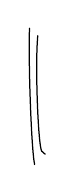
\begin{tikzpicture}[x=1cm,y=1cm,line width=.45pt,line cap=round]
\draw (0,0) .. controls (-.015,-.48) and (.025,-1.54) .. (.065,-1.73);
\draw (.105,-.095) .. controls (.070,-.48) and (.110,-1.48) .. (.155,-1.56) .. controls (.165,-1.58) and (.185,-1.59) .. (.200,-1.60);
\end{tikzpicture}}}
\margin{\unsure{rappelons qu'on suppose} $\pi$ \unsure{anabélien|nonabélien}
$(2g+\nu\geq3)$}
\[
1\longrightarrow\pi'\longrightarrow
\widehat{\widehat{\mathcal T}}(\pi,i)\longrightarrow
\unsure{\widehat{\widehat{\mathcal G}}}(\pi',i)\longrightarrow1
\]
ou encore
\[
1\longrightarrow\widehat{\pi}_{g,\nu-1}\longrightarrow
\widehat{\widehat{\mathcal T}}_{g,(\nu,\nu-1)}
\longrightarrow\unsure{\widehat{\widehat{\mathcal G}}}_{g,\nu-1}
\longrightarrow1
\]
qui contient la suite exacte
\[
1\longrightarrow\pi_{g,\nu-1}^{\unsure{*|+}}\longrightarrow
\mathcal T_{g,(\nu,\nu-1)}\longrightarrow
\unsure{\mathcal G}_{g,\nu-1}\longrightarrow1
\]
\unsure{comme|connue} sous\deleted{\unsure{particulière|partie dense}}, \unsure{suite|est} exacte.
Il est commode de travailler plutôt avec
\diagram{\begin{tikzcd}[ampersand replacement=\&,column sep=2.1em,row sep=3.0em]
1 \arrow[r,dash] \&
\pi_{g,\nu-1} \arrow[r,dash] \arrow[d,hook',no head] \&
\unsure{\mathcal T}_{g,\nu}^{!+} \arrow[r] \arrow[d,hook',no head] \&
\mathcal G_{g,\nu-1}^{!+} \arrow[r,dash] \arrow[d,hook',no head] \& 1 \\
1 \arrow[r,dash] \&
\widehat{\pi}_{g,\nu-1} \arrow[r] \arrow[d,equal] \&
\underset{\deleted{\unsure{\illegible{1}}}}{\widehat{\mathcal T}_{g,\nu}^{!+}}
\arrow[r] \arrow[d,hook',no head] \&
\widehat{\mathcal G}_{g,\nu-1}^{!+} \arrow[r,dash] \arrow[d,hook'] \& 1 \\
1 \arrow[r,dash] \&
\widehat{\pi}_{g,\nu-1} \arrow[r] \&
\widehat{\widehat{\mathcal T}}_{g,\nu}^{!} \arrow[r] \&
\widehat{\widehat{\mathcal G}}_{g,\nu-1}^{!} \arrow[r,dash] \& 1
\end{tikzcd}}

L'application $\unsure{\text{Prédiscrét}|\text{Prédiscrit}}^{+}(\pi)\longrightarrow
\unsure{\text{Prédiscrét}|\text{Prédiscrit}}^{+}(\pi')$ s'identifie donc à
$\widehat{\widehat{\mathcal T}}_{g,\nu}^{!}/\widehat{\mathcal T}_{g,\nu}^{!}$,
on lit sur le diagramme que c'est
$\simeq\widehat{\widehat{\mathcal G}}_{g,\nu-1}^{\unsure{!}\deleted{\unsure{+}}}/
\widehat{\mathcal G}_{g,\nu-1}^{!+}$,
d'où la bijectivité sur les ens des prédiscrétifications orientées.

Dans le groupe $\widehat{\widehat{\mathcal T}}_{g,\nu}^{!}=\mathcal T$,
on a un sous-groupe invariant $\widehat{\pi}_{g,\nu-1}=\pi'$,
et un sous-groupe $\Sigma$ $(\unsure{=|\longleftarrow}\widehat{\mathcal T}_{g,\nu}^{!+})$
\mspage{347}

\scanpage{349}

entre $\pi'$ et $\mathcal T$, \deleted{\unsure{donnant par}} \inserted{donnant} un ss-groupe $\Sigma'\simeq\mathcal T(\pi')$\inserted{$(=\unsure{\widehat{\mathcal G}^{!+}_{g,\nu-1}})$} dans $\unsure{\mathcal T'}=\mathcal T/\pi'$ $(\simeq\widehat{\widehat{\mathcal G}}^{!}_{g,\nu-1})$, et on sait bien qu'alors
\[
\mathcal T/\Sigma\simeq\mathcal T'/\Sigma',
\]
et \deleted{$\unsure{N(\Sigma)}$} que le normalisateur \inserted{$\mathcal N$,} de $\Sigma$ dans $\mathcal T$ est l'image inverse du normalisateur $\mathcal N'$ de $\Sigma'$ dans $\mathcal T'$, de sorte que $\mathcal N/\Sigma\simeq\mathcal N'/\Sigma'$, ce qui prouve ce qu'on voulait.

\uline{Corollaire} On a des \unsure{is.} canoniques
\[
\Gamma_{g,\nu}\xrightarrow{\sim}\Gamma_{g,\nu-1}\xrightarrow{\sim}\unsure{\cdots}\quad\deleted{\unsure{\Gamma_{g,0}}}
\]
\margin{On voit aussi que $\unsure{\Sigma|\Sigma^{!}}$ invariant dans $\unsure{\mathcal T|\widehat{\widehat{\mathcal T}}}$ équivaut à $\Sigma'$ invariant dans $\widehat{\widehat{\mathcal T}}'$}
de sorte que si $g\geq2$, on a \unsure{canoniqt} $\Gamma_{g,\nu}\simeq\Gamma_{g,0}$, d'autre part $\Gamma_{1,\nu}\simeq\Gamma_{1,1}$ $(g=1,\nu\geq1)$, $\Gamma_{0,\nu}\simeq\Gamma_{0,3}$ $(\nu\geq3)$.

\uline{NB} Le ``fait'' \deleted{\illegible{1}} admis est loin d'être évident --- même que $\widehat{\widehat{\mathcal T}}^{\unsure{!}}_{g,(\nu,\nu-1)}\longrightarrow\unsure{\widehat{\widehat{\mathcal T}}_{g,\nu-1}|\widehat{\widehat{\mathcal M}}_{g,\nu-1}}$ soit surjectif, ou que $\widehat{\widehat{\mathcal T}}_{g,(\nu,\nu-1)}\longrightarrow\widehat{\widehat{\mathcal G}}_{g,\nu-1}$ soit injectif, est loin d'être évident, et est peut-être tout à fait faux !

Le fait admis revient à un énoncé d'existence d'un foncteur \unsure{en} sens inverse ``forage des trous'', \unsure{qui|quid} en tout état de cause reste incompris.

\mspage{348}

\scanpage{350}
\mspage{177}

28. \uline{Changement de type} $(g,\nu)$ \unsure{(suite)} : \uline{\unsure{passage} à un rev. fini.}

Soit $\pi$ un groupe profini \inserted{à lacets} de type $(g,\nu)$, anabélien comme tjrs, $\pi'$ un ss-groupe d'indice fini. On sait (\unsure{ou on|on en} vérifie, par passage au cas discret) que \deleted{\illegible{1} \unsure{discrétifié}} \inserted{muni des} \unsure{traces} \unsure{sur|sous} $\pi$ des ss-groupes à \unsure{lacets} de $\pi$, $\pi'$ est un groupe à lacets.

\deleted{Si pour tout $i\in I(\pi)$, on considère un $L_i$, et les $\unsure{n}$ conjugués $\unsure{\operatorname{int}(g)}L_i$ \inserted{$=L_{i\alpha}$}, avec $g\in\pi\bmod\pi'$ $(n=[\pi:\pi']\unsure{\}},\ \deleted{\unsure{n}}\ \inserted{1\leq\alpha\leq n})$ \deleted{\unsure{comptés|compter} le nb de fois qu'une classe de conjugaison dans $\pi'$ du ss-groupe $\unsure{\operatorname{int}(g)}L_i$ est} \inserted{alors si $\unsure{d_{\alpha}|d_{i\alpha}}=[L_{i\alpha}:\unsure{L'_{i\alpha}|N'_{i\alpha}}\deleted{\unsure{\cap\pi'}}]$ \unsure{pour} $L'_{i\alpha}=L_{i\alpha}\cap\pi'$, alors} exactement $d_{i\alpha}$ parmi les $L'_{i\beta}$ \inserted{$(1\leq\beta\leq n)$} sont conjugués dans $\pi'$ à $L'_{i\alpha}$, et si on somme sur les classes de \unsure{conjugaison} distinctes des sous-groupes}

Les sous-groupes à lacets sont \unsure{aussi|ainsi} les \deleted{\unsure{les}} sous-groupes $L'$ tels que
\[
\text{a)}\quad L'=\operatorname{Centr}_{\pi}(L')\cap\pi'.
\]
\[
\text{b)}\quad L\unsure{=|:}\operatorname{Centr}_{\pi}(L')\text{ est un sous-groupe à \unsure{lacet} dans }\pi.
\]
On pose $d(L')=[L:L']$, et on a ainsi une fonction
\[
d:I'=I(\pi')\longrightarrow\mathbb N^*,
\]
et une application $I'\xrightarrow{\varphi}I$, telles que $\forall i\in I$, on ait
\[
\text{(1)}\qquad \sum_{\substack{i'\in I'\\\text{sur }i}}d(i')=n
\qquad (\text{\unsure{où|ici}}\ n=[\pi:\pi'])
\]
On aura la formule de Hurwitz
\[
\text{(2)}\qquad \deleted{\unsure{2g|2\alpha}}\ 2g'-2=n(2g-2)+\overbrace{\sum_{i'\in I'}(d(i')-1)}^{\inserted{n\operatorname{card}I-\operatorname{card}I'}}
\]
\mspage{349}
